\subsection{System Architecture}
The Horse Racing Tournament Management System is designed following a modern 3-tier software architecture. This architectural pattern guarantees a strict separation of concerns, scalability, and ease of maintenance by dividing the application into three distinct layers: the Presentation Layer, the Application Server Layer, and the Data Persistence Layer.

Figure \ref{fig:system_arch} illustrates the high-level system architecture and how data flows across these layers:
\begin{figure}[H]
    \centering
    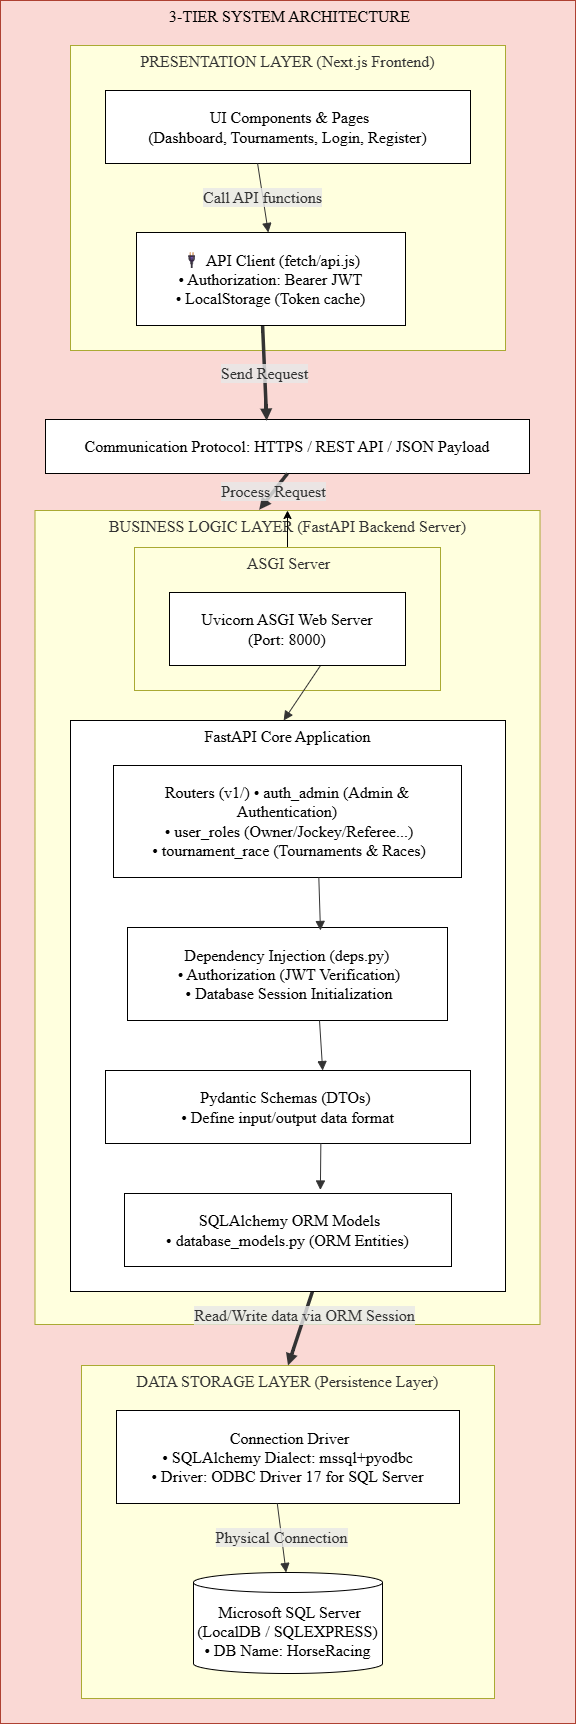
\includegraphics[width=0.75\textwidth, height=0.82\textheight, keepaspectratio]{figures/chuong4_diagram_chung/system_architecture.png}
    \caption{Overall System Architecture}
    \label{fig:system_arch}
\end{figure}

\begin{itemize}
    \item \textbf{Presentation Layer (Frontend):} Implemented using Next.js (React Framework). It runs directly inside the client's web browser, rendering interactive and responsive user interfaces (such as registration forms, tournament dashboards, scoreboards, and leaderboards). It communicates with the backend exclusively via HTTP requests carrying JSON payloads, passing JSON Web Tokens (JWT) for authentication.
    \item \textbf{Application Server Layer (Backend):} Built on FastAPI (Python). It is hosted on a high-performance ASGI server (Uvicorn). This layer exposes secure REST API endpoints, handles business logic (such as scheduling races, validating horse registrations, allocating referees, recording race violations, and computing points), performs user authentication, and coordinates transactions with the database.
    \item \textbf{Data Persistence Layer (Database):} Managed by Microsoft SQL Server (MSSQL). It stores the persistent relational data including user credentials, role definitions, horse profiles, registration records, tournament schedules, race results, and award distributions. It connects to the backend through SQLAlchemy ORM utilizing the \texttt{pyodbc} driver.
\end{itemize}

\subsection{Backend Architecture}
The backend application utilizes the FastAPI framework to provide a modular, performant, and secure API server. Figure \ref{fig:backend_arch} depicts the internal architectural layers of the backend system:

\begin{figure}[H]
    \centering
    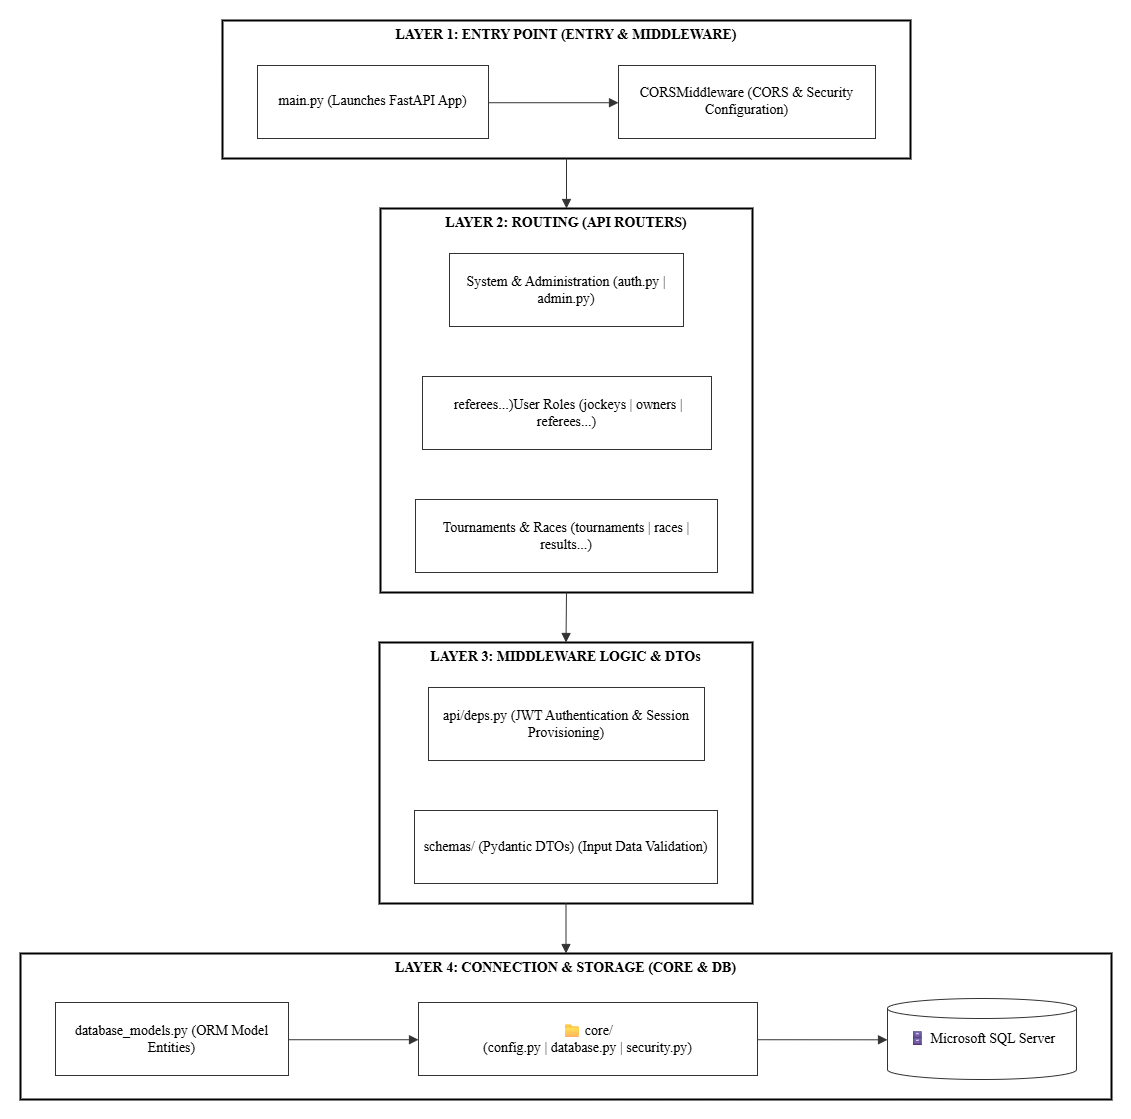
\includegraphics[width=0.95\textwidth]{figures/chuong4_diagram_chung/backend_architecture.png}
    \caption{FastAPI Backend Core Architecture}
    \label{fig:backend_arch}
\end{figure}

The backend processing flow is structured into the following operational stages:
\begin{enumerate}
    \item \textbf{Entry Point \& Security Middleware:} The application entry is defined in \texttt{main.py}. All incoming requests are filtered through \texttt{CORSMiddleware} to validate security origins and ensure safe cross-origin communication.
    \item \textbf{API Routing:} Requests are routed to specific endpoints under \texttt{/api/v1/} managed by modular routers (such as \texttt{auth}, \texttt{admin}, \texttt{user\_roles}, and \texttt{tournament\_race}).
    \item \textbf{Dependency Injection \& DTO Validation:} Request payloads are validated against Pydantic Schemas (Data Transfer Objects). Meanwhile, the dependency injection system in \texttt{deps.py} validates JWT authorization and provisions active SQL database sessions.
    \item \textbf{Core Logic \& ORM Mapping:} Validated requests are processed through business logic and mapped to relational database entities using SQLAlchemy ORM declarative models (\texttt{database\_models.py}).
    \item \textbf{Database Persistence:} SQLAlchemy executes the transactions against Microsoft SQL Server using the SQL Server connection string defined in \texttt{config.py} and database session helper in \texttt{database.py}.
\end{enumerate}

\subsection{Web Application Architecture}
The user interface is structured as a Single Page Application (SPA) using Next.js. Figure \ref{fig:web_arch} details the architectural layers and components of the Web Application:

\begin{figure}[H]
    \centering
    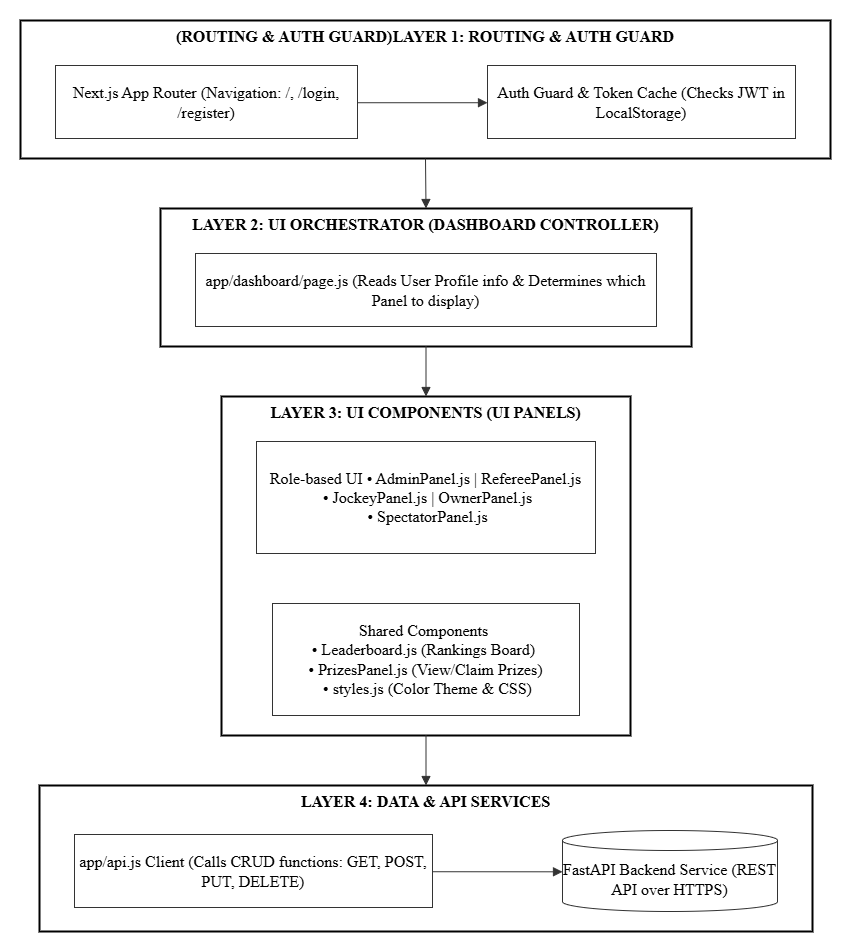
\includegraphics[width=0.95\textwidth]{figures/chuong4_diagram_chung/web_application_architecture.png}
    \caption{Next.js Web Application Frontend Architecture}
    \label{fig:web_arch}
\end{figure}

The frontend architectural workflow is organized as follows:
\begin{enumerate}
    \item \textbf{Routing \& Authentication Guard:} Next.js App Router controls client-side navigation. The \texttt{Auth Guard} inspects the browser's local storage for a valid JWT token. Unauthenticated users are redirected to the Login or Register routes, while authenticated users are allowed access to the dashboard.
    \item \textbf{Dashboard Controller:} Located in \texttt{dashboard/page.js}, it fetches the authenticated user's profile details. It dynamically checks the user's role (Admin, Jockey, Horse Owner, Referee, Spectator) to determine which UI component to mount.
    \item \textbf{Role-based UI Panels:} Specialized interfaces are mounted dynamically based on role configurations (such as \texttt{AdminPanel}, \texttt{JockeyPanel}, \texttt{OwnerPanel}, \texttt{RefereePanel}, or \texttt{SpectatorPanel}).
    \item \textbf{Shared Components \& Styles:} Common interface sections like \texttt{Leaderboard.js} and \texttt{PrizesPanel.js} are imported by multiple roles, applying uniform CSS styling definitions.
    \item \textbf{API Client Layer:} The centralized HTTP client utility in \texttt{api.js} communicates with the FastAPI Backend server via async \texttt{fetch} operations, managing request headers and auth tokens.
\end{enumerate}
